\documentclass[11pt,a4paper]{article}

\usepackage[margin=2.35cm,headheight=15pt]{geometry}
\usepackage[T1]{fontenc}
\usepackage[utf8]{inputenc}
\usepackage{lmodern}
\usepackage{microtype}
\usepackage{amsmath,amssymb}
\usepackage{booktabs,tabularx,array}
\usepackage{enumitem}
\usepackage{xcolor}
\usepackage{fancyhdr}
\usepackage{titlesec}
\usepackage{tcolorbox}
\usepackage{tikz}
\usetikzlibrary{arrows.meta,positioning,fit}
\usepackage[hidelinks]{hyperref}
\usepackage{lastpage}
\usepackage{ragged2e}

\definecolor{SSBlue}{HTML}{17365D}
\definecolor{SSLight}{HTML}{EAF0F7}
\definecolor{SSGray}{HTML}{5A6470}
\definecolor{SSLine}{HTML}{B8C5D4}
\definecolor{SSGreen}{HTML}{2F6B4F}
\definecolor{SSRed}{HTML}{8A3B3B}

\pagestyle{fancy}
\fancyhf{}
\fancyhead[L]{\small\textsc{Semantic Secrets}}
\fancyhead[R]{\small\textsc{Research Description}}
\fancyfoot[C]{\small\thepage}
\renewcommand{\headrulewidth}{0.4pt}
\renewcommand{\footrulewidth}{0pt}

\titleformat{\section}{\Large\bfseries\color{SSBlue}}{\thesection}{0.7em}{}
\titleformat{\subsection}{\large\bfseries\color{SSGray}}{\thesubsection}{0.7em}{}
\titlespacing*{\section}{0pt}{1.6em}{0.7em}
\titlespacing*{\subsection}{0pt}{1.2em}{0.5em}

\setlist[itemize]{leftmargin=1.5em,itemsep=0.25em,topsep=0.35em}
\setlist[enumerate]{leftmargin=1.75em,itemsep=0.35em,topsep=0.35em}
\setlength{\parindent}{0pt}
\setlength{\parskip}{0.55em}
\renewcommand{\arraystretch}{1.2}

\newtcolorbox{keybox}[1][]{
  colback=SSLight,
  colframe=SSBlue,
  boxrule=0.8pt,
  arc=2mm,
  left=3mm,right=3mm,top=2.5mm,bottom=2.5mm,
  #1
}

\newtcolorbox{statusbox}[1][]{
  colback=white,
  colframe=SSLine,
  boxrule=0.6pt,
  arc=1.5mm,
  left=3mm,right=3mm,top=2mm,bottom=2mm,
  #1
}

\newcommand{\code}[1]{\texttt{#1}}
\newcommand{\Aset}{\mathcal{A}}

\begin{document}

\hypersetup{pageanchor=false}
\begin{titlepage}
\centering
\vspace*{2.0cm}
{\Huge\bfseries\color{SSBlue} Semantic Secrets\par}
\vspace{0.4cm}
{\LARGE Research Description and Technical Direction\par}
  \vspace{0.25cm}
  {\large EuroS\&P 2027 target and October dataset status\par}
\vspace{1.0cm}
\rule{0.82\textwidth}{0.7pt}
\vspace{1.0cm}

\begin{minipage}{0.84\textwidth}
\begin{keybox}
\centering
\textbf{Research in one sentence.}\par\medskip
Semantic Secrets studies whether independently reconstructed visual concepts can yield stable and discriminative canonical semantic credentials, whether the fuzzy acceptance region induced by approximate matching remains resistant to realistic and AI-assisted guessing, and whether that predicate can be privately verified without exposing a reusable semantic template, a practical offline guess-testing oracle, or cross-domain linkage.
\end{keybox}
\end{minipage}

\vfill
  {\large Working Draft -- status reviewed 26 October 2026\par}
\vspace{0.2cm}
{\small Internal research-direction document; not a publication manuscript\par}
\vspace{0.3cm}
  {\small Repository basis: \code{franciscobecerra97/Semantic-Secrets-v1}, technical direction through commit \code{90fe344}\par}
\end{titlepage}
\hypersetup{pageanchor=true}

\setcounter{tocdepth}{1}
\tableofcontents
\newpage

\section{Abstract}

Most authentication systems rely on exact reproduction of a secret value or proof of exact cryptographic possession. Semantic Secrets studies a different primitive: \emph{approximate semantic reconstruction}. An intended concept may be expressed through different natural-language prompts and independently generated into different images, yet those realizations may preserve enough canonical visual semantics to authenticate as equivalent. The project therefore does not treat the prompt or the generated image as the credential. The prompt is a reconstruction interface, the image is a transient reconstruction medium, probabilistic perception produces bounded evidence, and deterministic compilation converts that evidence into a canonical semantic graph.

Approximate semantic authentication changes the security object. Instead of one exact accepted value, the verifier induces a fuzzy acceptance region containing multiple semantic alternatives. This creates a central trade-off: a predicate that is too strict rejects legitimate independent reconstructions, while a predicate that is too tolerant enlarges the set of alternatives an attacker can submit. The project therefore measures the complete accepted region under increasingly informed and AI-assisted attackers rather than treating random false-acceptance rate as sufficient security evidence.

A second, independent problem is privacy. A semantic graph, policy, protected record, or authentication transcript can potentially reveal the underlying concept, support database-only candidate validation, leak the structure of the acceptance policy, enable adaptive probing, or permit cross-service linkage. Semantic correctness and cryptographic privacy are therefore evaluated through separate gates. Only if the semantic primitive remains viable does the project compare and implement mature private-verification constructions.

The research proceeds sequentially: modular visual extraction, independent generative reconstruction, system-derived mandatory/tolerant policy evaluation, acceptance-region attacks, private verification, and finally an end-to-end prototype and held-out evaluation. The active extraction contract composes the immutable v3.0 architecture, the v3.1 pipeline/resource/support amendment, the v3.2 project-authored-ground-truth correction, and the v3.3 development-calibration rule. Human memorability, usability, natural secret choice, and superiority to passwords or passkeys are explicit non-goals. Client-side computational practicality is measured rather than assumed; impractical local requirements are a legitimate limitation or negative result rather than a reason to move secret-bearing processing to an untrusted cloud.

\section{Motivation and Research Justification}

\subsection{The motivation is no longer password memorability}

The project originally grew from an intuitive password-oriented idea: people may be able to recall a visual idea more flexibly than an exact high-entropy string. That intuition helped motivate early exploration, but it is not the claim that the current technical research can support. The present programme contains no human-subject study and therefore cannot establish that visual concepts are easier to remember, that users can reconstruct them over long time periods, or that the resulting system is more usable than passwords or passkeys.

The stronger and more accurate motivation is a security question about the transition from \emph{exact reproduction} to \emph{approximate semantic reconstruction}.

Traditional authentication can be idealised as accepting one enrolled value:
\begin{equation}
  \Aset(s)=\{s\}.
\end{equation}

Semantic Secrets instead asks whether one intended concept can be independently reconstructed into different textual and visual realizations that still produce sufficiently compatible canonical semantics. For a controlled intended concept $C$:
\begin{align}
  C &\rightarrow P_1 \rightarrow I_1 \rightarrow O_1 \rightarrow S_1,\\
  C &\rightarrow P_2 \rightarrow I_2 \rightarrow O_2 \rightarrow S_2,
\end{align}
where normally $P_1\neq P_2$ and $I_1\neq I_2$, but the technical hypothesis is that $S_1$ and $S_2$ remain compatible under a frozen authentication predicate while targeted semantic alternatives remain distinguishable.

\begin{keybox}
\textbf{Primary motivation.} The project investigates what happens when authentication accepts semantic equivalence rather than one exact representation: whether the resulting credential can be reconstructed reliably, whether its full acceptance region remains difficult to enter, and whether the fuzzy predicate can be verified privately.
\end{keybox}

\subsection{Why generative AI and images remain in the design}

The image generator is not justified as a memorability mechanism and generated pixels are not treated as entropy. Instead, the generator acts as an experimental \emph{semantic reconstruction and normalisation boundary}. Different natural-language descriptions of the same intended concept may produce visibly different images. The project asks whether those independently generated visual realizations preserve enough underlying structure for canonical semantic comparison.

The roles are therefore deliberately separated:

\begin{center}
\begin{tabularx}{0.92\textwidth}{>{\bfseries}l X}
Prompt $P$ & reconstruction interface; not the credential \\
Generated image $I$ & transient reconstruction medium; not the credential \\
Observations $O$ & bounded probabilistic visual evidence with provenance/confidence \\
Canonical graph $S$ & deterministic security-sensitive semantic representation \\
Acceptance region $\Aset(S)$ & operational secret surface: all semantics that the verifier accepts \\
\end{tabularx}
\end{center}

Thus the current scientific hypothesis is not that images are better passwords. It is that independent generative reconstruction may preserve a sufficiently stable visual-semantic core to support a new fuzzy authentication primitive.

\subsection{The acceptance region is the central security problem}

Let the frozen semantic decision be $\mathsf{Accept}(S,S')$. The accepted semantic region is
\begin{equation}
  \Aset(S)=\{S' : \mathsf{Accept}(S,S')=1\}.
\end{equation}

An attacker does not need the original prompt, the original image, or the exact enrolled graph. Any $S'\in\Aset(S)$ is sufficient. Consequently, the main matching problem is inseparable from the main security problem:

\begin{center}
\begin{tabular}{rcl}
\textbf{too strict} & $\longrightarrow$ & legitimate independent reconstructions fail,\\[0.3em]
\textbf{too tolerant} & $\longrightarrow$ & attackers gain more accepted semantic alternatives.
\end{tabular}
\end{center}

This is why the project treats the complete acceptance region, rather than a nominal atom count or random false-acceptance rate, as the relevant security object.

\subsection{Why privacy is a separate contribution}

Even a stable and discriminative semantic credential may be unsafe to store or verify naively. A plaintext graph can directly expose semantic content. A deterministic record may allow a database attacker to test semantic guesses offline. Policy metadata can reveal which attributes are mandatory, and deterministic records or transcripts may permit cross-service linkage.

Therefore the project separates two questions:

\begin{enumerate}
  \item \textbf{Semantic correctness:} does the extraction/reconstruction/policy pipeline accept legitimate independent reconstructions and reject important alternatives?
  \item \textbf{Cryptographic privacy:} can the same frozen decision be evaluated while limiting template, policy, record, transcript, compromise, and linkage leakage?
\end{enumerate}

Passing one does not imply the other. Private computation cannot make an easily reachable semantic region strong, while good semantic discrimination does not automatically make stored state private.

\section{Central Research Question and Goals}

\subsection{Central research question}

\begin{keybox}
\centering
\textbf{Can independently reconstructed visual concepts yield stable and discriminative canonical semantic credentials whose complete acceptance region remains sufficiently resistant to realistic and AI-assisted guessing, and whose authentication predicate can be privately verified without exposing a reusable semantic template, practical offline guess-testing oracle, or cross-domain linkage?}
\end{keybox}

\subsection{Operational goals}

The project has six operational goals:

\begin{enumerate}
  \item \textbf{Visual-semantic extraction.} Determine which semantic fact types can be recovered reliably enough from generated images to become credential material.
  \item \textbf{Independent reconstruction.} Determine whether different prompts and generation randomness for the same controlled concept produce compatible canonical semantics while targeted alternatives remain distinguishable.
  \item \textbf{Policy-aware matching.} Determine whether a system-derived split between mandatory anchors $M$ and tolerant semantics $T$ improves the reconstruction/security trade-off over simpler and VSA-style baselines.
  \item \textbf{Acceptance-region security.} Measure how easily random, frequency-informed, partial-information, near-secret, AI-assisted, and adaptive attackers can enter the accepted region under explicit finite budgets.
  \item \textbf{Private verification.} Identify and evaluate a construction that reproduces the frozen semantic decision while limiting semantic disclosure, database-only validation, policy leakage, adaptive leakage, and cross-domain linkability under explicit compromise assumptions.
  \item \textbf{Practicality.} Quantify computation, memory, storage, bandwidth, latency, deployment assumptions, and failure modes without silently moving secret-bearing processing to an untrusted cloud provider.
\end{enumerate}

\subsection{Contribution hypotheses}

These are prospective hypotheses, not present claims.

\begin{description}[style=nextline,leftmargin=1.5em,labelindent=0pt]
  \item[\textbf{C1 -- Technical reconstructability of visual-semantic credentials.}]
  Independently generated images of the same controlled concept may yield compatible canonical semantics while remaining separable from targeted semantic alternatives.

  \item[\textbf{C2 -- System-derived policy-aware semantics.}]
  A deterministic policy $\Pi(S)=(M,T)$ may preserve benign reconstruction variation while rejecting security-critical semantic differences better than dense, global-overlap, or closest feasible VSA-style baselines.

  \item[\textbf{C3 -- Acceptance-region security.}]
  The reachability of the fuzzy semantic region can be characterised using K0--K3 knowledge classes, finite budgets, frequency information, semantic neighbours, AI assistance, and adaptive one-bit feedback.

  \item[\textbf{C4 -- Private and unlinkable verification.}]
  A construction-specific protocol may evaluate the frozen semantic predicate while limiting template leakage, database-only offline validation, policy/transcript leakage, and cross-domain linkage under explicit assumptions.
\end{description}

C1 and C2 are enabling contributions. If the constructive path survives, C3 and C4 are expected to carry the strongest security/privacy contribution.

\section{Target System and Credential Model}

The invariant technical path is

\begin{center}
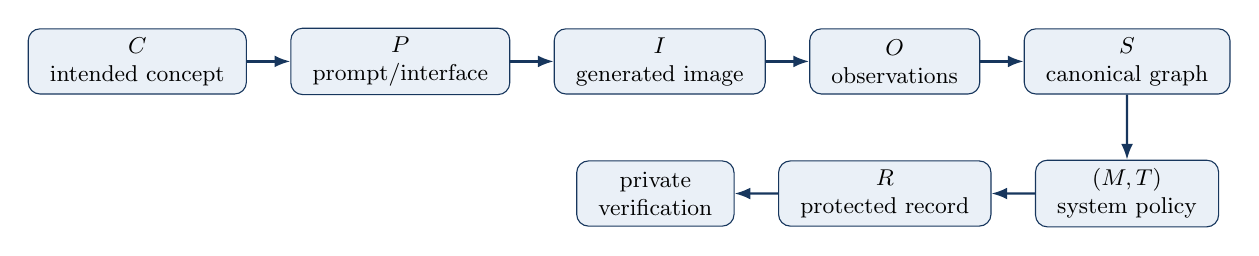
\begin{tikzpicture}[scale=0.92,transform shape,node distance=5mm and 6mm, every node/.style={font=\small},
  box/.style={draw=SSBlue, rounded corners=1.5mm, fill=SSLight, align=center, minimum height=9mm, inner xsep=3mm},
  arr/.style={-{Latex[length=2mm]}, thick, draw=SSBlue}]
\node[box] (c) {$C$\\intended concept};
\node[box, right=of c] (p) {$P$\\prompt/interface};
\node[box, right=of p] (i) {$I$\\generated image};
\node[box, right=of i] (o) {$O$\\observations};
\node[box, right=of o] (s) {$S$\\canonical graph};
\node[box, below=9mm of s] (mt) {$(M,T)$\\system policy};
\node[box, left=of mt] (r) {$R$\\protected record};
\node[box, left=of r] (v) {private\\verification};
\draw[arr] (c)--(p);
\draw[arr] (p)--(i);
\draw[arr] (i)--(o);
\draw[arr] (o)--(s);
\draw[arr] (s)--(mt);
\draw[arr] (mt)--(r);
\draw[arr] (r)--(v);
\end{tikzpicture}
\end{center}

The strongest target architecture keeps $P$, $I$, $O$, plaintext $S$, and raw learned representations inside a trusted client. Public algorithms, models, schemas, thresholds, and policies are not treated as secrets. The authentication infrastructure should receive only construction-specific protected material and the explicitly allowed protocol output/metadata.

The current extraction architecture explicitly separates probabilistic perception from deterministic credential mechanics:
\begin{equation}
  I \xrightarrow{\mathsf{Observe}} O \xrightarrow{\mathcal{C}_s} S.
\end{equation}

$\mathsf{Observe}$ may produce detections, attributes, unary actions, binary interactions/spatial relations, scenes, bounding boxes, confidence values, provenance, abstentions, and typed component failures. The deterministic compiler owns schema validation, canonical IDs, deduplication, sorting, count derivation, geometry-derived facts, inverse-relation normalisation, versioning, typed failures, and canonical serialization.

The candidate language $L_{\mathrm{visual}}$ is intentionally broad. Only semantic atom types that independently satisfy the frozen capability criteria in both controlled and naturalistic strata may enter the credential language $L_{\mathrm{cred}}\subseteq L_{\mathrm{visual}}$.

\section{Experimental Programme}

The research is deliberately sequential. Later phases cannot compensate for a failed earlier gate.

\subsection{P9-v3B -- modular component capability and $L_{\mathrm{cred}}$ eligibility}

This is the next empirical phase. It does \emph{not} yet test authentication or independent reconstruction. It asks whether the semantic evidence required by the future credential can be extracted reliably and compiled deterministically.

The executable v3.1 shortlist is exactly:
\begin{enumerate}
  \item \textbf{Grounding DINO Tiny + SigLIP2 Base}: open-set object localisation plus closed-label semantic scoring;
  \item \textbf{EGTR + SigLIP2 Base}: graph-native object/relation extraction plus independent attribute/scene scoring.
\end{enumerate}

The future capability data has two strata, with 120 final images in each:
\begin{itemize}
  \item \textbf{Controlled}: project-authored geometric/composited fixtures with project-authored closed-label entities, normalized boxes, and semantic atoms for exact objects, counts, geometry, and compiler edge cases.
  \item \textbf{Naturalistic}: project-authored prompt/seed plans rendered by the frozen local generator, followed by project-authored closed-label reference specifications for the final visible images without consulting any perception-model output.
\end{itemize}

P9-v3B has no human participants or annotators. Before perception inference, all 240 final image hashes, scenario specifications, manifest rows, and deterministic positive/applicable-negative support opportunities must pass their audits and be bound into \code{ground-truth-freeze-v3.2.0}. The reference data may never be derived from Grounding DINO, SigLIP2, EGTR, or later validation output.

The phase measures type-level precision, recall, F1, coverage, abstention/failure, repeatability, uncertainty, latency, RAM/VRAM, and exact compiler correctness through at least 320 deterministic cases. Development thresholds are selected only after threshold-independent score capture, using the fixed inclusive $0.00,0.01,\ldots,1.00$ grid and the frozen v3.3 entity-first, task-local, both-strata ranking rule. Entity scopes are frozen before downstream scoring; EGTR predicate/connectivity thresholds are fitted jointly; each SigLIP2 task is fitted independently; count and geometry receive no fitted threshold; and neither validation data nor cross-pipeline pooling may influence calibration. Integrated development replay and \code{threshold-freeze-v3.3.0} precede formal authorisation and validation.

Gate V3-A1 requires one complete pipeline to yield a non-trivial eligible $L_{\mathrm{cred}}$ containing entities plus at least two additional semantic types, including a structural type, while satisfying the frozen reliability, repeatability, failure, and resource criteria. Eligible types cannot be unioned across pipelines.

\subsection{P9-v3C -- independent visual reconstruction}

Only after V3-A1 passes does the project test the central reconstruction hypothesis on separate preregistered data:
\begin{equation}
  P_1\rightarrow I_1\rightarrow S_1
  \qquad \text{versus} \qquad
  P_2\rightarrow I_2\rightarrow S_2,
\end{equation}
where $P_1$ and $P_2$ are semantically equivalent controlled descriptions and generation randomness is independent.

Gate V3-A2 evaluates enrolment eligibility, false rejection, targeted-neighbour false acceptance, random false acceptance, same-vs-near discrimination, failure, uncertainty, and the frozen policy interface. This phase may establish technical reconstruction viability, but not memorability, entropy, privacy, or real-world usability.

\subsection{P10 -- system-derived mandatory/tolerant policy}

After a constructive V3-A2, the project evaluates the policy
\begin{equation}
  \Pi(S)=(M,T),
\end{equation}
where $M$ contains mandatory/discriminative anchors and $T$ contains bounded-tolerance secondary semantics. The policy is system-derived, deterministic, versioned, and fitted only on authorised development evidence; users do not manually nominate the primary anchors in the technical study.

The proposed design is compared against dense similarity, global fuzzy overlap, and the closest feasible VSA-style semantic-policy baseline. Gate V2-B asks whether the policy materially improves the reconstruction/security trade-off without post-hoc held-out tuning.

\subsection{P11 -- acceptance-region and budgeted attackers}

P11 evaluates C3 over the complete accepted region. It freezes K0--K3 strategies and explicit budgets for random, frequency-informed, semantic-neighbour, partial-information, LLM-assisted, generator/VLM-assisted, and adaptive attackers where justified.

For strategy $Q$, budget $B$, knowledge class $K_i$, and observable view $V$:
\begin{equation}
  \mathsf{Succ}(Q,B,K_i,V)=
  \Pr[\exists j\le B: S'_j\in\Aset(S)].
\end{equation}

The evaluation reports success@budget, guesses-to-success, duplicates, uncertainty, cost, and online/offline access separately. Gate V2-C determines the surviving positioning: standalone, second factor, policy-constrained/restricted, measurement/negative, or stop.

\subsection{P12--P14 -- private verification}

Only if the semantic region remains viable does the project define the ideal private functionality and compare mature construction families such as OPRF/VOPRF, PSI and circuit-PSI variants, secure computation, fuzzy extractor/PAKE alternatives, and encrypted similarity methods.

The objective is not to invent a new cryptographic primitive. The objective is to identify a construction-specific privacy property that improves meaningfully over plaintext/hash-style baselines while reproducing the frozen semantic decision. A small surviving set is implemented as proof of concept, one direction is selected, and the selected verifier is hardened with domain separation, session binding, replay/downgrade handling, explicit compromise analysis, transcript minimisation, adaptive-query analysis, and unlinkability tests.

\subsection{P15--P20 -- integration, held-out evidence, manuscript, and artifact}

A constructive path culminates in an end-to-end prototype, one frozen held-out evaluation, deterministic figures/statistics, the evidence-backed EuroS\&P manuscript, a reproducible research artifact, and a final submission audit. The gate order remains:

\begin{center}
\small
V2-N $\rightarrow$ historical V2-A failure $\rightarrow$ V3-A1 $\rightarrow$ V3-A2 $\rightarrow$ V2-B $\rightarrow$ V2-C $\rightarrow$ V2-D $\rightarrow$ V2-E $\rightarrow$ V2-F.
\end{center}

No later phase may bypass a failed earlier gate.

\section{Expected Results and Valid Outcomes}

The project is designed so that scientifically useful evidence does not require the constructive hypothesis to succeed fully.

\subsection{Constructive outcome}

A strong positive result would establish a defensible subset of the following:
\begin{enumerate}
  \item at least one modular extractor supports a non-trivial, reliable $L_{\mathrm{cred}}$ within the declared measured resource envelope;
  \item independent generated realizations of the same controlled concept preserve enough canonical semantics to support technical reconstruction;
  \item the system-derived $M/T$ policy improves the reconstruction/security trade-off over simpler and VSA-style baselines;
  \item budgeted K0--K3 and AI/adaptive attackers do not make the accepted region trivially reachable under the claimed use setting;
  \item a private construction materially reduces template leakage, database-only candidate validation, or linkability relative to plaintext/hash baselines;
  \item the complete pipeline is practical enough for an interactive or explicitly qualified deployment setting.
\end{enumerate}

\subsection{Restricted positive outcome}

The primitive may be technically defensible but unsuitable for universal primary authentication. Evidence may instead support a second factor, policy-constrained credential, restricted/high-value setting, or another bounded deployment. For example, K0/K1 resistance could be acceptable while strong K3 knowledge remains a documented limitation, or the client-side computation could be too heavy for ubiquitous use but acceptable in a narrower setting.

\subsection{Negative or measurement outcome}

A failed gate is evidence, not permission to retune. Scientifically useful negative outcomes include:
\begin{itemize}
  \item current modular extractors cannot recover a sufficiently rich and reliable credential language;
  \item independent generative reconstruction is too unstable;
  \item the tolerance required for reconstruction makes the acceptance region too easy to enter;
  \item the $M/T$ policy offers no meaningful improvement over simpler baselines;
  \item private matching is possible but does not materially improve the relevant compromise/privacy property;
  \item the selected verifier is too slow or leaks too much policy/transcript metadata;
  \item local secret-bearing extraction or generation requires impractical hardware under the intended trust model.
\end{itemize}

A negative result may support a measurement/limitations paper or stop the constructive path entirely.

\section{Prototype Design}

The final prototype should demonstrate the scientific pipeline without making a user interface part of the contribution. A CLI/API is sufficient.

\begin{center}
\begin{tabularx}{\textwidth}{>{\bfseries}p{0.28\textwidth} X}
\toprule
Module & Responsibility \\
\midrule
Local generator & Produce independent images from natural-language reconstruction inputs under frozen/versioned generation settings. \\
Observation pipeline & Produce bounded detections, attributes, actions/interactions, relations, scenes, confidence/provenance, abstentions, and typed failures. \\
Semantic compiler & Deterministically build a canonical graph or typed failure; own schema, IDs, deduplication, counts, geometry, inverse normalisation, ordering, and serialization. \\
Policy engine & Derive $M/T$, thresholds, eligibility, and version metadata using only authorised development evidence. \\
Plaintext reference matcher & Implement the exact frozen predicate against which every private construction is checked. \\
Privacy protocol layer & Protect enrolment state and privately reproduce the reference decision under an explicit leakage/compromise model. \\
Authentication service & Manage account/session context, protocol messages, rate limits, replay/version controls, and final decisions. \\
Optional privacy/key service & Hold independent key/share material only if the selected construction requires explicit non-collusion or threshold assumptions. \\
Attack framework & Generate K0--K3, AI-assisted, semantic-neighbour, inversion, linkage, compromise, and adaptive-query evaluations. \\
Experiment runner & Execute frozen manifests, hashes, caches, resource telemetry, statistical analyses, and reproducibility checks. \\
CLI/API demonstrator & Show end-to-end enrolment and authentication without becoming the scientific core. \\
\bottomrule
\end{tabularx}
\end{center}

The prototype should enforce the trusted-client boundary for secret-bearing prompt/image/semantic processing and should fail closed on malformed graphs, unsupported operators, missing mandatory anchors, version mismatch, replay/downgrade ambiguity, and protocol errors.

\section{Scope}

The current research includes:
\begin{itemize}
  \item reconstructable semantic authentication from independently generated visual realizations;
  \item modular visual perception and deterministic canonical semantic compilation;
  \item technical reconstruction stability under controlled paraphrase, seed, style, and layout variation;
  \item derivation and evaluation of a system-derived mandatory/tolerant policy;
  \item random and targeted false-acceptance/false-rejection behaviour;
  \item acceptance-region reachability and finite-budget K0--K3 attackers;
  \item AI-assisted semantic guessing and adaptive one-bit probing;
  \item template inversion, database-only candidate validation, and cross-domain/account linkage;
  \item private-verification constructions with explicit stored-state, transcript, policy, and compromise leakage;
  \item performance, memory, storage, bandwidth, latency, and deployment assumptions;
  \item reproducible project-authored/safely licensed experimental artifacts;
  \item evidence-backed positioning that may ultimately be standalone, second-factor, constrained or restricted, negative or measurement, or stop.
\end{itemize}

\section{Non-Goals and Claim Boundaries}

The project must not use technical experiments as a substitute for evidence about human behaviour. The present work does \emph{not} aim to establish:

\begin{itemize}
  \item that visual concepts are easier to remember than passwords;
  \item long- or short-term human recall, memorability, usability, preference, accessibility, or real-world authentication time;
  \item that users naturally select high-entropy semantic concepts;
  \item that generated pixels add credential entropy;
  \item that Semantic Secrets is necessarily a universal password replacement;
  \item superiority to passwords, passkeys, biometrics, hardware authenticators, or other mature authentication systems;
  \item firstness for semantic, image-independent, VLM-based, policy-based, or generative graphical authentication;
  \item novelty merely from object/attribute/count/spatial rules, $M/T$ notation, or standard primitives such as OPRF, PSI, PAKE, MPC, FHE, or fuzzy extraction;
  \item privacy, unlinkability, irreversibility, or offline resistance merely because semantic values are hashed, salted, encoded, or encrypted;
  \item protection after total compromise unless the selected construction explicitly supports such a claim;
  \item that a third-party cloud GPU is a normal trusted participant in the deployed architecture.
\end{itemize}

Human memorability and natural secret-choice behaviour remain possible future human-subject questions only if the technical primitive first proves worth studying with people.

\section{The Research Narrative}

The project should be explained in the following order.

\begin{enumerate}
  \item \textbf{Exact authentication has one representation problem; semantic authentication creates a region problem.} Most authentication expects an exact value or exact possession. Semantic reconstruction intentionally allows multiple representations of one intended concept.
  \item \textbf{Generative reconstruction is the experimental bridge.} Different natural-language descriptions are independently rendered into different images. The image generator acts as a reconstruction/normalisation boundary, not a source of memorability or entropy.
  \item \textbf{Canonical semantics make the idea testable.} Probabilistic visual evidence is compiled deterministically into a typed graph so that representation errors, semantic errors, and serialization errors can be measured separately.
  \item \textbf{Tolerance creates the central security tension.} The verifier must tolerate benign reconstruction variation, but every tolerated alternative can enlarge the attacker's winning set.
  \item \textbf{The full acceptance region must therefore be attacked.} Security is measured under explicit budgets and increasingly informed K0--K3/AI/adaptive strategies, not inferred from random FAR alone.
  \item \textbf{Privacy remains independent.} Even a good predicate may reveal a semantic template or enable offline candidate testing/linkage. The project therefore evaluates private verification separately and only after semantic viability.
  \item \textbf{Practicality determines positioning rather than being assumed.} The evidence decides whether the primitive belongs in standalone authentication, a factor/constrained setting, a restricted deployment, a measurement paper, or nowhere.
\end{enumerate}

\begin{keybox}
\textbf{The story is therefore not:} ``AI-generated images are easier-to-remember passwords.''\par\medskip
\textbf{The story is:} ``What security and privacy properties emerge when authentication moves from exact secret reproduction to reconstructable semantic equivalence?''
\end{keybox}

\section{EuroS\&P 2027 Target}

The active target is the 12th IEEE European Symposium on Security and Privacy, Madrid, 5--9 July 2027. Mandatory title/abstract/author/conflict/topic registration is 25 November 2026 AoE, followed by full-paper submission on 2 December 2026 AoE. The supplied IEEE conference template uses A4 and a 13-page body limit; references, appendices and submission acknowledgments are additional. Essential security evidence and proactive harm analysis remain in the body, with Data Availability and anonymous AI-use acknowledgments. The official 2027 CFP and the repository's venue requirements govern policy; older PoPETs issue plans are historical.

The narrative leads with acceptance-region security under independent reconstruction, then separately examines private verification. Research gates and contribution meanings are unchanged. On 13 November, review whether actual completed evidence can support a finished paper. The current timetable is high risk; missing a cycle is preferable to weakening criteria or presenting an unfinished system as validated.

\section{Current Status}

As of the repository state reviewed on 15 October 2026, the latest project work remains the prospective preparation completed in August 2026:

\begin{enumerate}
  \item \textbf{Historical v1 (P0--P7):} earlier text/image representations and matching assumptions were tested. P6 found poor targeted-neighbour separation in the frozen v1 matcher, and P7 found no material benefit from the tested v1 image pathways over paired text pathways. These results remain immutable formative evidence.
  \item \textbf{P8:} novelty was refreshed against VSA and broader prior work. Gate V2-N passed only with narrowed claims around the complete composition of independent generative reconstruction, typed canonical semantics, system-derived policy, acceptance-region analysis, and private verification.
  \item \textbf{P9-v2:} the frozen monolithic ``image $\rightarrow$ general VLM $\rightarrow$ exact complete credential JSON'' architecture failed its schema-validity gate. This rejects that architecture only; it is not evidence that visual semantics are universally infeasible.
  \item \textbf{P9-v3A:} a new v3.0 architecture separated learned observations from deterministic compilation and preregistered new capability/reconstruction gates without running a v3 experiment.
  \item \textbf{P9-v3A.1:} the prospective v3.1 audit selected EGTR as the graph-native comparator, preserved Grounding DINO + SigLIP2 as the other pipeline, clarified measured-resource rules, and froze support opportunities. Its historical two-human annotation prerequisite was later superseded before any v3 output.
  \item \textbf{Narrative and execution preparation (26 August 2026):} active documentation was aligned around reconstructable semantic authentication, acceptance-region security, and private verification. The deterministic v3 compiler, isolated two-environment RunPod design, provenance guards, and guarded execution/export workflow were prepared. The compiler matrix passes 320/320 locally, but this is engineering evidence only and must be rerun in the locked image.
  \item \textbf{P9-v3A.2 (28 August 2026):} the mismatched human-annotation dependency was prospectively replaced with project-authored, closed-label, model-blind reference specifications and a hash-bound ground-truth freeze. P9-v3B now has no human participants or annotators.
  \item \textbf{Execution-readiness audit (29 August 2026):} deterministic data materialisation, persistent model sessions, telemetry, evaluation, Gate computation, formal authorisation, resume checks, and provenance-complete export were implemented. The audit correctly left project-authored scenario/prompt content as an unresolved input rather than inventing it.
  \item \textbf{P9-v3A.3 (29 August 2026):} the missing prospective threshold method was frozen and implemented: fixed-grid, development-only, entity-first, task-local calibration; deterministic fallback; offline replay; validation isolation; and a provenance-bound threshold freeze. This amendment did not select any empirical threshold or start an experiment.
\end{enumerate}

\begin{statusbox}
\textbf{P9-v3B data preparation is in progress; formal perception evaluation has not started.} All 240 capability images and 120 controlled references exist. The remaining 120 naturalistic references must be authored without perception predictions; complete manifest/support audits and the ground-truth freeze remain pending. Remote SD-Turbo generation was requested, but actual endpoint weights/settings are unattested. Compiler and runtime tests are engineering evidence. The current audit found one-to-one entity-scoring and moved-manual-path defects to correct before model evaluation. No v3 capability, reconstruction, authentication, attack-resistance or private-verification result exists. Acquisition and inference retain their existing authorization and freeze requirements.
\end{statusbox}

\section{Immediate Direction}

The immediate objective is \textbf{not} to implement the final authentication system or cryptography. It is to determine whether the representation layer is viable at all.

The next permitted empirical sequence, once explicitly authorised, is:

\begin{enumerate}
  \item obtain the applicable authorization for model acquisition and perception inference; image generation already occurred under the separate October decision;
  \item finish the model-output-blind reference work off the GPU: images/plans and controlled records already exist; author the 120 naturalistic final-image records and audit support;
  \item verify retained image/receipt hashes and remote-generation provenance, and disclose that actual endpoint weights/settings are unattested; do not regenerate or select favorable replacements;
  \item build and audit the 240-row manifest and deterministic support-opportunity table, then create \code{ground-truth-freeze-v3.2.0};
  \item acquire only the frozen Grounding DINO Tiny, SigLIP2 Base, and EGTR artifacts after licence, revision, hash, checkpoint-layout, and provenance checks;
  \item build/use the immutable container, rerun all 320 compiler cases, record the GPU environment, and run only the bounded engineering smoke permitted after the ground-truth freeze;
  \item capture development entity scores, fit and freeze entity scopes, capture downstream scores, perform the frozen offline component calibration, replay the integrated development tree, and create \code{threshold-freeze-v3.3.0};
  \item create the provenance-bound formal authorisation, run validation and its single frozen repeat, evaluate Gate V3-A1, and derive $L_{\mathrm{cred}}$ separately for each complete pipeline;
  \item if V3-A1 fails, stop the visual constructive path or preregister a genuinely new reframe; if it passes, separately preregister P9-v3C and test independent reconstruction under Gate V3-A2;
  \item only a constructive V3-A2 unlocks P10; policy value, acceptance-region attacks, private functionality/protocol work, integration, held-out evaluation, manuscript, and artifact phases remain gated in that order.
\end{enumerate}

The most important near-term question is therefore:

\begin{keybox}
\centering
\textbf{Can the project obtain a non-trivial, reproducible visual-semantic credential language from independently validated modular observations within the declared local-compute envelope?}
\end{keybox}

Until that question is answered, the final security/privacy architecture remains a hypothesis rather than an implementation target.

\section{What the Final Paper Should Ultimately Say}

If the constructive path survives all gates, the paper should ultimately tell the following story:

\begin{keybox}
Authentication normally relies on exact reproduction or exact cryptographic possession. Semantic Secrets studies a different primitive in which one intended concept may be independently reconstructed into different prompts and visual realizations that compile into compatible canonical semantics. Because approximate matching induces a non-singleton acceptance region, the verifier must balance legitimate reconstruction tolerance against the attacker's ability to find any accepted semantic alternative. We therefore measure the complete acceptance region under finite-budget knowledgeable and AI-assisted attackers rather than relying on random false-acceptance rate alone. We then evaluate whether the same frozen fuzzy predicate can be privately verified without exposing a reusable semantic template, practical database-only guess-testing oracle, policy structure, or cross-domain linkage. The resulting system is evaluated end to end under explicit compromise and practicality assumptions.
\end{keybox}

The strongest paper positioning should lead with C3 and C4 if the evidence supports them: acceptance-region security and construction-specific private verification. C1 and C2 should be presented as the enabling system mechanisms that make those questions possible.

The final paper should not claim that AI images are better passwords, that people remember semantic concepts better than strings, or that the system must replace passkeys/passwords. Instead, it should make a narrower and stronger contribution: a disciplined empirical and systems study of a reconstructable semantic authentication primitive, the security consequences of its induced acceptance region, the privacy consequences of storing/verifying a structured fuzzy credential, and the practical conditions under which such a primitive is or is not viable.

If the evidence instead supports only a restricted or negative result, the paper should say that clearly. A coherent final paper may conclude that the primitive works only in a constrained factor setting, that knowledgeable attackers make the region too weak for standalone use, that private verification fails to provide meaningful compromise resistance, or that local computation is impractical. The paper story must follow the strongest surviving evidence, not the original product intuition.

\section{Research Compass}

For day-to-day project decisions, the following compact mental model should remain stable:

\begin{center}
\begin{tabularx}{0.95\textwidth}{>{\bfseries}p{0.32\textwidth} X}
What is being studied? & A reconstructable semantic authentication primitive, not an easier-to-remember password. \\
What is reconstructed? & An intended semantic concept through different prompts and independently generated images. \\
What is the credential? & The canonical semantic representation under a frozen policy; operationally, the complete accepted region. \\
Why is matching hard? & Legitimate variation requires tolerance, but tolerance expands attacker alternatives. \\
Why is privacy hard? & Structured semantic state can reveal meaning, enable offline candidate validation, leak policy, or create linkage. \\
What must happen before cryptography? & Extraction, independent reconstruction, policy value, and acceptance-region security must pass their gates. \\
Where should secret-bearing AI run? & Inside the trusted client for the strongest claim; research GPUs are laboratory infrastructure, not automatically deployment components. \\
What happens next? & Complete naturalistic references and freeze the existing 240-image capability dataset, then execute the fixed P9-v3B score/calibration/validation sequence; only a V3-A1 pass unlocks P9-v3C. \\
What is not claimed? & Human memorability/usability, semantic entropy in pixels, password/passkey superiority, firstness, or privacy from hashing/encryption alone. \\
\end{tabularx}
\end{center}

\vfill
\begin{center}
\small\color{SSGray}
This document is an internal research-direction synthesis intended to keep the project goal, evidence sequence, architecture, scope, and claim boundaries visible while implementation evolves.
\end{center}

\end{document}
